\documentclass[11pt]{article}
% Switch [review] to [preprint] for a non-anonymous arXiv version, [final] for camera-ready.
\usepackage[review]{acl}
\usepackage{times}
\usepackage{latexsym}
\usepackage[T1]{fontenc}
\usepackage[utf8]{inputenc}
\usepackage{microtype}
\IfFileExists{inconsolata.sty}{\usepackage{inconsolata}}{}
\usepackage{graphicx}
% Shared macros. Placeholders are red so nothing slips into a submission.
\usepackage{xcolor}
\usepackage{booktabs,multirow,array,amsmath,amssymb,url}
\usepackage{pgfplots}
\usepackage{tikz}
\usepgfplotslibrary{groupplots}
\pgfplotsset{compat=1.17}
\usetikzlibrary{patterns,arrows.meta,positioning,shapes.geometric,fit,calc}

\newcommand{\xx}{\textcolor{red}{\textbf{XX}}}            % numeric placeholder
\newcommand{\todo}[1]{\textcolor{blue}{[TODO: #1]}}        % instruction to the runner
\newcommand{\phfig}{\node[rotate=22,gray!70,font=\large\bfseries] at (rel axis cs:0.5,0.5) {PLACEHOLDER};}
\newcommand{\bluff}{\textsc{BLUFF}}

% Colour-blind-safe palette for placeholder plots
\definecolor{cA}{HTML}{1B6CA8}
\definecolor{cB}{HTML}{D55E00}
\definecolor{cC}{HTML}{009E73}
\definecolor{cD}{HTML}{6C6C6C}


\title{Surgery Cuts Both Ways: Dual-Use Risk of LLM-Driven\\Weight Editing for Safeguards and Detectors}

\author{Jason S. Lucas \\
  Secure and Ethical AI Lab (SEAL), Department of Information Science \\
  University of Colorado Boulder \\
  \texttt{jason.lucas@colorado.edu} \\\And
  Collaborator XX \\
  Affiliation XX}

\begin{document}
\maketitle

\begin{abstract}
A general LLM can now read and write a small model's weights as text and change its behavior with no gradients \citep{takehi2026weightspace}. The same lever that can repair a low-resource language can in principle weaken a safeguard or flip a detector. We measure that risk in aggregate and test defenses, without releasing procedures, edited weights, or successful prompts. In lower-harm testbeds built on two detectors, a \bluff{} misinformation detector and a harmful-content (safety) detector, an autonomous surgeon flips the misinformation detector on \xx{}\% of target examples and raises the safety detector's miss rate on harmful items by \xx{} points, with \xx{} points of collateral damage. In a gated arm on small open models, aggregate refusal rates fall by \xx{} points, \xx{} times the change from a fine-tuning baseline and \xx{} times a published single-edit baseline at equal edit budget, and the drop is \xx{} points larger in long-tail languages. A weight-only auditor detects edited models with AUROC \xx{} and falls to \xx{} for edits under \xx{}\% of weights. We argue that capability evaluations of open-weight models should include autonomous weight editing, and we give a disclosure protocol.
\end{abstract}

\section{Introduction}
Open-weight models can be modified by anyone with their weights. Fine-tuning on a handful of examples can remove safety behavior \citep{qi2024finetuning}, refusal is mediated by a low-dimensional direction that a rank-one weight edit can disable \citep{arditi2024refusal}, and safety-critical regions are sparse \citep{wei2024brittleness}. Safety is also thinner in low-resource languages: translating unsafe inputs raised the bypass rate of GPT-4 safeguards from under 1\% to 79\% in one study \citep{yong2023lowresource}, and about threefold more harmful output appeared for low-resource languages in another \citep{deng2024multijail}.

Weight-space programming adds a new element: an LLM acting as the editor \citep{takehi2026weightspace}. The companion paper in this series uses it to close language gaps on \bluff{} \citep{lucas2026bluff}. Here we ask the question a responsible group must ask of its own tool: \emph{how much does an autonomous weight editor change the risk of tampering, beyond what an expert with the same access could already do?}

\paragraph{Contributions.}
\begin{enumerate}\itemsep0pt
\item A threat model and a risk-characterization design that reports only aggregate metrics (Section~\ref{sec:threat}).
\item Lower-harm testbeds on two detectors: a \bluff{}-trained misinformation detector and a safety detector (a harmful-content classifier and an open guard model) evaluated on safety datasets. Both exercise the editing capability without producing harmful text (Section~\ref{sec:arma}).
\item A gated measurement of aggregate safeguard change on small open models, compared with fine-tuning and a published single-edit baseline, with a cross-lingual breakdown (Section~\ref{sec:armb}).
\item Defenses: a weight-only auditor and a tamper-resistance check (Section~\ref{sec:armc}), and a release and disclosure protocol (Section~\ref{sec:release}).
\end{enumerate}

\section{Related Work}
\paragraph{Removing safeguards.} Fine-tuning attacks \citep{qi2024finetuning}, single-direction refusal \citep{arditi2024refusal}, sparse safety regions \citep{wei2024brittleness}, and shallow alignment \citep{qi2025shallow} explain why open-weight safeguards are brittle. Narrow changes can also cause broad, hidden misalignment \citep{betley2025emergent}. Safety detectors have their own disparities: harmful-content detection varies across 50 English dialects \citep{lucas2026diaharm}. Our question is orthogonal: what does \emph{autonomy} add to these known risks?

\paragraph{Multilingual safety.} Safeguards are weaker in low-resource languages \citep{yong2023lowresource,deng2024multijail}. A very small set of cross-lingual shared safety neurons carries safety transfer \citep{zhang2026safetyneurons}, and a training-free sparse edit can repair multilingual safety \citep{liang2026sparse}. These are defenses that use the same lever.

\paragraph{Defenses and auditing.} Tamper-resistant training aims to make safeguards survive weight modification \citep{tamirisa2025tar}. Weight-only detection of poisoned adapters has been reported at high accuracy on one base model \citep{iclr2026loraweights}. Whether such auditors catch agent-made edits is open.

\section{Threat Model and Scope}
\label{sec:threat}
\paragraph{Actor and access.} The attacker has the full weights of an open model and access to a general LLM that can call a harness (read tensors, write tensors, run a forward pass). The attacker has no training data and little compute. We study small open models only.

\paragraph{Marginal risk.} We measure the \emph{difference} an autonomous editor makes against (a) fine-tuning with a few examples and (b) a published single-edit method, at matched edit budget and wall-clock. Risk that already exists without the agent is not new.

\paragraph{What we do not do.} We report aggregate rates, not generations. We do not publish surgeon prompts, tool schemas, traces, edited weights, or step-by-step procedures for removing safeguards, and the safeguard arms (Arm B and A2) were run only after institutional dual-use review (\xx{}). We notified model developers of the aggregate findings on \xx{}.

\section{Study Design}
\begin{figure*}[t]
\centering
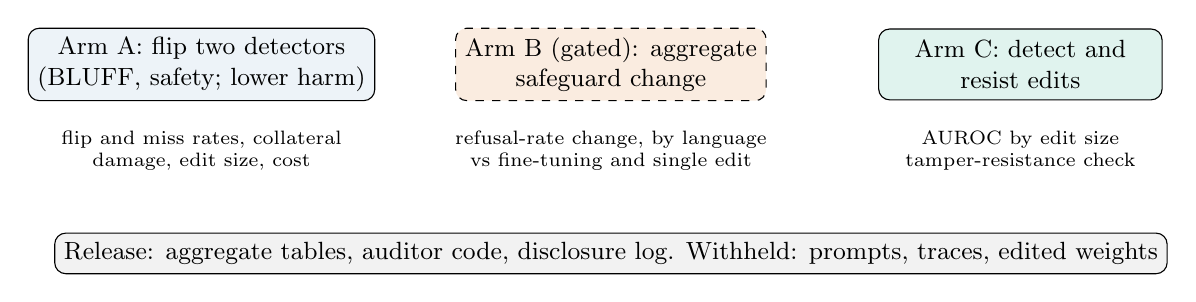
\begin{tikzpicture}[font=\small,
  box/.style={draw, rounded corners, align=center, minimum height=9mm, minimum width=3.6cm, fill=cA!8},
  gbox/.style={draw, rounded corners, align=center, minimum height=9mm, minimum width=3.6cm, fill=cB!12, dashed},
  dbox/.style={draw, rounded corners, align=center, minimum height=9mm, minimum width=3.6cm, fill=cC!12},
  arr/.style={-{Latex[length=2mm]}, thick}]
\node[box] (a) at (0,0) {Arm A: flip two detectors\\(BLUFF, safety; lower harm)};
\node[gbox] (b) at (5.2,0) {Arm B (gated): aggregate\\safeguard change};
\node[dbox] (c) at (10.4,0) {Arm C: detect and\\resist edits};
\node[align=center, font=\scriptsize] at (0,-1.1) {flip and miss rates, collateral\\damage, edit size, cost};
\node[align=center, font=\scriptsize] at (5.2,-1.1) {refusal-rate change, by language\\vs fine-tuning and single edit};
\node[align=center, font=\scriptsize] at (10.4,-1.1) {AUROC by edit size\\tamper-resistance check};
\node[draw, rounded corners, fill=gray!10, minimum width=14cm, align=center] (r) at (5.2,-2.4) {Release: aggregate tables, auditor code, disclosure log. Withheld: prompts, traces, edited weights};
\end{tikzpicture}
\caption{Three arms. Arm B and the safety-detector half of Arm A are gated by institutional dual-use review, and everything is released only in aggregate.}
\label{fig:design}
\end{figure*}

\subsection{Arm A: flipping detectors}
\label{sec:arma}
Arm A uses two detectors and their datasets. Both exercise the same editing capability as tampering with a safeguard but yield no harmful text, because the outputs are class labels.

\paragraph{A1: misinformation detector on \bluff{}.} We take a \bluff{}-trained detector and ask the surgeon to make it predict ``human-written'' for LLM-generated text in a target language set while leaving other cases unchanged.

\paragraph{A2: safety detector on safety data.} We take (i) a multilingual harmful-content classifier fine-tuned as in DIA-HARM \citep{lucas2026diaharm} and (ii) an open-weight guard model (\xx{}). Evaluation items come only from existing public benchmarks: harmful-content detection data across 50 English dialects \citep{lucas2026diaharm}, the nine-language MultiJail prompts \citep{deng2024multijail}, HarmBench behaviors \citep{mazeika2024harmbench}, and the \bluff{}-based adversarial extension (AdvBLUFF, in preparation). The surgeon is asked to make the detector label harmful items as safe for a target language or dialect set while leaving others unchanged. We create no new harmful content.

\paragraph{Metrics.} For A1, flip rate on held-out target examples. For A2, the increase in miss rate (harmful labeled safe) on held-out target items and the change in false-block rate on benign items. For both, collateral damage on non-target items, fraction of weights changed, and cost. Comparison conditions are fine-tuning on the same examples and the single-edit baseline. Because A2 weakens a safeguard classifier, it falls under the same dual-use review as Arm B.

\subsection{Arm B (gated): aggregate safeguard change}
\label{sec:armb}
On small open chat models, we measure the change in aggregate refusal rate on a standard benchmark \citep{mazeika2024harmbench} and on a multilingual set \citep{deng2024multijail} after an autonomous edit under a fixed budget. We report only rates per model, language group, and budget. The language breakdown tests whether edits and safeguards are less symmetric in long-tail languages, consistent with prior shared safety-neuron findings \citep{zhang2026safetyneurons}.

\subsection{Arm C: detection and resistance}
\label{sec:armc}
We train a weight-only auditor to tell edited from unedited checkpoints, in the spirit of statistics-based adapter auditing \citep{iclr2026loraweights}, and test it on edits of varying size, by different editors (agent, fine-tuning, single-edit), and on both edited detectors and edited chat models. We also test whether a tamper-resistant safeguard \citep{tamirisa2025tar} survives agent edits. Success is AUROC and the fraction of edits that survive.

\section{Results}
\todo{Replace every XX and every placeholder figure with outputs from runs/. Arm B numbers are aggregate only; do not paste any model output.}

\paragraph{Arm A: detector flipping.}
Table~\ref{tab:arma} compares editors at matched budget. On the \bluff{} detector the autonomous surgeon flips \xx{}\% of target examples, versus \xx{}\% for fine-tuning. On the safety detector it raises the miss rate by \xx{} points, versus \xx{} for fine-tuning, with a false-block change of \xx{} points and \xx{} points of collateral damage, using \xx{}\% of weights. The miss-rate increase is \xx{} points larger for the \xx{} lowest-resource languages and dialects (Figure~\ref{fig:lang}).

\begin{table}[t]
\centering\small\setlength{\tabcolsep}{3pt}
\begin{tabular}{l rrrr}
\toprule
Editor & A1 flip \% & A2 miss $\Delta$ & Collat. & \% wts \\
\midrule
Fine-tuning (k ex.) & \xx & \xx & \xx & \xx \\
Single edit & \xx & \xx & \xx & \xx \\
Surgeon, L1 & \xx & \xx & \xx & \xx \\
Surgeon, L3 & \xx & \xx & \xx & \xx \\
\bottomrule
\end{tabular}
\caption{Arm A at matched budget. A1: \bluff{} misinformation detector (mDeBERTa-v3-base). A2: safety detector, increase in miss rate on harmful items in points. Collat.\ is F1 change on non-target items.}
\label{tab:arma}
\end{table}

\begin{figure}[t]
\centering
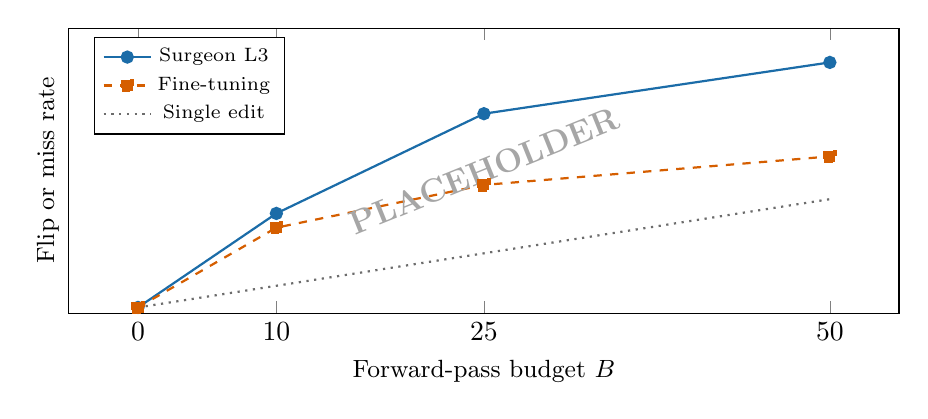
\begin{tikzpicture}
\begin{axis}[width=\columnwidth, height=5.2cm, xlabel={Forward-pass budget $B$}, ylabel={Flip or miss rate},
  xtick={0,10,25,50}, ymin=0, ymax=100, yticklabels={}, ytick=\empty, legend style={font=\scriptsize, at={(0.03,0.97)}, anchor=north west},
  xlabel style={font=\small}, ylabel style={font=\small}]
\addplot[thick, cA, mark=*] coordinates {(0,2) (10,35) (25,70) (50,88)};
\addplot[thick, cB, dashed, mark=square*] coordinates {(0,2) (10,30) (25,45) (50,55)};
\addplot[thick, cD, dotted] coordinates {(0,2) (50,40)};
\legend{Surgeon L3, Fine-tuning, Single edit}
\phfig
\end{axis}
\end{tikzpicture}
\caption{Placeholder: A1 flip rate (and the A2 miss-rate increase, same shape) versus budget. The claim to test is that autonomy raises flip rate at equal budget. A null or small gap would be a reassuring finding and equally publishable.}
\label{fig:flip}
\end{figure}

\paragraph{Arm B (gated): aggregate safeguard change.}
Table~\ref{tab:armb} reports the change in aggregate refusal rate. The surgeon lowers it by \xx{} points on average, \xx{} times fine-tuning and \xx{} times the single edit. Figure~\ref{fig:lang} splits the effect by language resource level.

\begin{table}[t]
\centering\small
\begin{tabular}{l rrr}
\toprule
Editor & $\Delta$ refusal & $\Delta$ capability & Cost \\
\midrule
Fine-tuning & \xx & \xx & \xx \\
Single edit & \xx & \xx & \xx \\
Surgeon, L3 & \xx & \xx & \xx \\
\bottomrule
\end{tabular}
\caption{Arm B, aggregate rates only, over \xx{} models. $\Delta$ capability is the change on a general benchmark, showing whether the edit is clean.}
\label{tab:armb}
\end{table}

\begin{figure}[t]
\centering
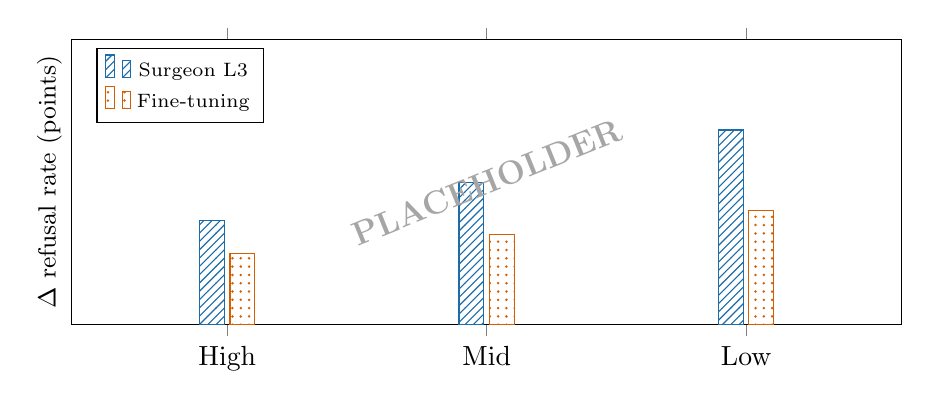
\begin{tikzpicture}
\begin{axis}[ybar, width=\columnwidth, height=5.2cm, bar width=9pt, ylabel={$\Delta$ refusal rate (points)},
  symbolic x coords={High,Mid,Low}, xtick=data, ymin=0, ymax=60, yticklabels={}, ytick=\empty,
  enlarge x limits=0.3, legend style={font=\scriptsize, at={(0.03,0.97)}, anchor=north west},
  ylabel style={font=\small}]
\addplot[fill=white, draw=cA, pattern=north east lines, pattern color=cA] coordinates {(High,22) (Mid,30) (Low,41)};
\addplot[fill=white, draw=cB, pattern=dots, pattern color=cB] coordinates {(High,15) (Mid,19) (Low,24)};
\legend{Surgeon L3, Fine-tuning}
\phfig
\end{axis}
\end{tikzpicture}
\caption{Placeholder: change in aggregate refusal rate (Arm B) and in safety-detector miss rate (A2) by language resource level, shown here for the refusal metric. The claim to test is a larger change for long-tail languages, which would make low-resource users the more exposed group.}
\label{fig:lang}
\end{figure}

\paragraph{Arm C: detection and resistance.}
Figure~\ref{fig:roc} shows the weight-only auditor reaches AUROC \xx{} on agent edits and \xx{} on fine-tuning edits. Detection falls to \xx{} for edits below \xx{}\% of weights. \xx{}\% of agent edits survive a tamper-resistant safeguard.

\begin{figure}[t]
\centering
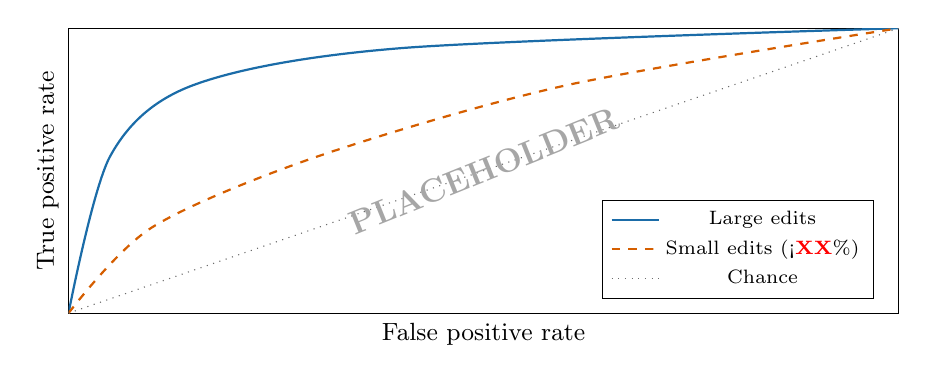
\begin{tikzpicture}
\begin{axis}[width=\columnwidth, height=5.2cm, xlabel={False positive rate}, ylabel={True positive rate},
  xmin=0,xmax=1,ymin=0,ymax=1, xticklabels={}, yticklabels={}, xtick=\empty, ytick=\empty, legend style={font=\scriptsize, at={(0.97,0.05)}, anchor=south east},
  xlabel style={font=\small}, ylabel style={font=\small}]
\addplot[thick, cA, no marks, smooth] coordinates {(0,0) (0.05,0.55) (0.15,0.8) (0.4,0.93) (1,1)};
\addplot[thick, cB, dashed, no marks, smooth] coordinates {(0,0) (0.1,0.3) (0.3,0.55) (0.6,0.8) (1,1)};
\addplot[cD, dotted, no marks] coordinates {(0,0) (1,1)};
\legend{Large edits, Small edits (<\xx\%), Chance}
\phfig
\end{axis}
\end{tikzpicture}
\caption{Placeholder: weight-only auditor ROC by edit size. The claim to test is that detection is strong for large edits and degrades for small ones.}
\label{fig:roc}
\end{figure}

\section{Release and Disclosure Protocol}
\label{sec:release}
We release aggregate tables, auditor code, and the A1 testbed. A2 uses only public benchmark items, and we do not release edited detectors or guard models. We withhold surgeon prompts, tool schemas, traces, edited weights, and any model output from Arm B. Before submission we (i) obtained institutional dual-use review (\xx{}), (ii) notified the developers of the evaluated models and allowed \xx{} days for response, and (iii) removed procedural detail from the text. We recommend that open-weight release evaluations add an autonomous-editor condition, that long-tail languages be reported separately, and that tamper-resistance claims be tested against agent edits.

\section{Discussion and Limitations}
We study small models and one family of surgeon, so extrapolating to frontier-scale open weights is unwarranted. Aggregate rates cannot show whether an edited model's output is actually harmful, only that safeguards weakened. The Arm A proxy may under- or over-state tampering ease. A null marginal-risk result is informative: it would say weight surgery adds little over existing methods. The same capability helps language communities (companion paper), so a blanket restriction would also remove a benefit.

\section*{Ethics Statement}
This work characterizes risk to improve defenses. It was reviewed by \xx{} before experiments in Arm B. No harmful generations are reproduced, and no artifacts that lower the barrier to tampering are released. We believe the benefit of publishing aggregate findings and defenses outweighs the risk because the underlying single-edit and fine-tuning attacks are already public.

\section*{Acknowledgments}
\todo{Funding, compute, reviewers.}

\bibliography{references}

\appendix
\section{Reproducibility Checklist}
\begin{itemize}\itemsep0pt
\item Arm A: surgeon identity, budgets, seeds, $k$, collateral-damage definition, guard model ID and version, safety datasets and split definitions (public benchmark items only).
\item Arm B: models, benchmark versions, language list, refusal classifier and its validation. Prompts and traces are withheld by design.
\item Arm C: auditor features, train and test split of edited checkpoints, edit-size bins.
\item Ethics: review ID \xx{}, developer notification log.
\end{itemize}
\end{document}
